%\documentclass{beamer}
\documentclass[trans,draft]{beamer} %TODO remove trans,draft



\mode<presentation>
{
	\usetheme{Frankfurt}
	
	
	\definecolor{maincolor}{rgb}{1,0.39,0}
%	\setbeamercolor{alerted text}{fg=maincolor!65!red!90!black}
	\setbeamercolor{alerted text}{fg=maincolor!75!yellow}
	\setbeamercolor{palette primary}{fg=white,bg=maincolor}
%	\setbeamercolor{palette quaternary}{fg=maincolor,bg=white}
	\setbeamercolor{palette quaternary}{fg=white,bg=maincolor!75!black}
	\setbeamercolor{structure}{fg=maincolor,bg=maincolor!50}
	
%	\setbeamerfont{alerted text}{series=\bf}
	
	
	\setbeamercovered{transparent}
}


\usepackage[english]{babel}

\usepackage{amsmath}
\usepackage{amssymb}
\usepackage{xspace}
\usepackage{colonequals}
\usepackage{times}

\usepackage{tikz}
\usetikzlibrary{shapes,positioning,arrows,calc,fit,backgrounds}
\pgfdeclarelayer{foreground layer}
\pgfsetlayers{background,main,foreground layer}

\usepackage[utf8]{inputenc}
\usepackage[T1]{fontenc}






%====================================================================
% Identifiers
%====================================================================

\newcommand{\atoms}{\ensuremath{\mathcal{A}}\xspace}
\newcommand{\literals}{\ensuremath{\mathcal{L}}\xspace}% TODO .: this is usually a symbol for language !!!

%\newcommand{\rule}{\ensuremath{r}\xspace}
\newcommand{\prog}{\ensuremath{P}\xspace}
\newcommand{\unfounded}{\ensuremath{\Upsilon}\xspace}

\newcommand{\pospart}[1]{\ensuremath{{#1}^{+}}\xspace}
\newcommand{\negpart}[1]{\ensuremath{{#1}^{-}}\xspace}

\newcommand{\nrule}{\ensuremath{\rho}\xspace}
\newcommand{\nprog}{\ensuremath{\Pi}\xspace}
\newcommand{\snprog}{\ensuremath{\nprog_{\#}}\xspace}
\newcommand{\rwprog}[1]{\ensuremath{\nprog_{#1}}\xspace}
\newcommand{\syn}{\ensuremath{\mathcal{S}}\xspace}
\newcommand{\sem}{\ensuremath{\mathbb{S}}\xspace}

\newcommand{\sealion}{{SeaLion}\xspace}
\newcommand{\clasp}{{Clasp}\xspace}
\newcommand{\gringo}{{Gringo}\xspace}
\newcommand{\dlv}{{DLV}\xspace}
\newcommand{\lana}{{\sc{Lana}}\xspace}
\newcommand{\aspdoc}{{ASPDoc}\xspace}
\newcommand{\kara}{{Kara}\xspace}
\newcommand{\ape}{{APE}\xspace}
\newcommand{\aspide}{{ASPIDE}\xspace}
\newcommand{\igrom}{{iGROM}\xspace}



%====================================================================
% Commands
%====================================================================

\newenvironment{myitemi}{\begin{itemize}\def\mite{\item}}{\end{itemize}}
% \newenvironment{myitemi}{\def\mite{}}{}

\makeatletter
\newcommand{\breakinglist}[1]{%
	\@tempcnta=0
	\@for\@ii:=#1\do{%
		\@insertbreakingcomma
		{\@ii}
	}%
}
\def\@insertbreakingcomma{%
	\ifnum \@tempcnta = 0 \else , \linebreak[1] \fi
	\advance\@tempcnta\@ne
}
\makeatother


\newcommand{\set}[1]{\ensuremath{\left\{{#1}\right\}}\xspace}
\newcommand{\bset}[1]{\ensuremath{ \{ \breakinglist{#1} \} }\xspace}
\newcommand{\seq}[1]{\ensuremath{\left[{#1}\right]}\xspace}
\newcommand{\tuple}[1]{\ensuremath{\langle {#1} \rangle}\xspace}
\newcommand{\btuple}[1]{\ensuremath{\langle \breakinglist{#1} \rangle}\xspace}
\newcommand{\prj}[2]{\ensuremath{\pi_{#1}\textit{(}{#2}\mathit{)}}\xspace}
\newcommand{\abs}[1]{\ensuremath{|{#1}|}\xspace}
\newcommand{\modulo}{\ensuremath{\mathrm{\ mod\ }}\xspace}
\newcommand{\setcomp}[2]{\ensuremath{\{#1 \mid #2\}}}
\newcommand{\multiset}[1]{\ensuremath{\dot{\{}#1\dot{\}}}}
\newcommand{\kleene}[0]{\ensuremath{^*}}
\newcommand{\familycomp}[2]{\ensuremath{(#1 \mid #2)}}

\newcommand{\basicG}{\ensuremath{G_B}\xspace}
% \newcommand{\ntr}[1]{\ensuremath{\texttt{<}\textit{#1}\texttt{>}}\xspace}
% \newcommand{\ntr}[1]{\ensuremath{\texttt{<}\textit{#1}\texttt{>}}\xspace}
\newcommand{\ntr}[1]{\texttt{<}\textit{#1}\texttt{>}}
% \newcommand{\ntr}[1]{\ensuremath{\mathtt{<}\textit{#1}\mathtt{>}}\xspace}
% \newcommand{\trm}[1]{\ensuremath{\texttt{``}\textit{#1}\texttt{''}}\xspace}
\newcommand{\trm}[1]{\ntr{#1}}
\newcommand{\opt}[1]{\ensuremath{[{#1}]}\xspace}
\newcommand{\rpt}[1]{\ensuremath{\{{#1}\}}\xspace}
\newcommand{\rptplus}[1]{\ensuremath{\dot\{{#1}\dot\}}\xspace}
\newcommand{\toCFGrules}[1]{\ensuremath{\tau\textit{(}{#1}\mathit{)}}\xspace}
\newcommand{\Gext}[6]{\ensuremath{\textit{ext(}{#1},\linebreak[1]{#2},\linebreak[1]{#3},\linebreak[1]{#4},\linebreak[1]{#5},\linebreak[1]{#6}\mathit{)}}\xspace}
% \newcommand{\str}[2]{\ensuremath{\text{\guillemotleft}\textit{{#1}-{#2}}\text{\guillemotright}}\xspace}
\newcommand{\str}[2]{\ensuremath{\mathtt{\ll}\textit{{#1}-{#2}}\mathtt{\gg}}\xspace}
% \newcommand{\code}[1]{\text{``\texttt{#1}''}}
% \newcommand{\code}[1]{\text{"\texttt{#1}"}}
% \newcommand{\code}[1]{\ensuremath{\texttt{``{#1}''}}\xspace}
\newcommand{\code}[1]{\ensuremath{\texttt{\bfseries{#1}}}\xspace}
% \newcommand{\code}[1]{\text{\guillemotleft\texttt{#1}\guillemotright}}
\newcommand{\funid}[1]{\ensuremath{\mathit{#1}}\xspace}
\newcommand{\algid}[1]{\mbox{\sc #1}}

\newcommand{\sneg}{\ensuremath{\neg}\xspace}
\newcommand{\naf}{\ensuremath{\mathbf{not}}\xspace}
\newcommand{\hor}{\ensuremath{\texttt{|}}\xspace}
\newcommand{\rif}{\ensuremath{\leftarrow}\xspace}

\newcommand{\domain}[1]{\ensuremath{{D_{#1}}}\xspace}
\newcommand{\satisfiers}[1]{\ensuremath{C_{#1}}\xspace}
\newcommand{\head}[1]{\ensuremath{H\mathrm{(}{#1}\mathrm{)}}\xspace}
\newcommand{\body}[1]{\ensuremath{B\mathrm{(}{#1}\mathrm{)}}\xspace}
\newcommand{\pbody}[1]{\ensuremath{B^\mathrm{+}\mathrm{(}{#1}\mathrm{)}}\xspace}
\newcommand{\nbody}[1]{\ensuremath{B^\mathrm{-}\mathrm{(}{#1}\mathrm{)}}\xspace}
% \newcommand{\proj}[2]{\ensuremath{{#1}|_{#2}}}
\newcommand{\proj}[2]{\ensuremath{{#1}\cap {#2}}}
\newcommand{\flpred}[2]{\ensuremath{{#1}^{#2}}\xspace}
\newcommand{\activerules}[2]{\flpred{#2}{#1}}

\newcommand{\AS}[1]{\ensuremath{\mathit{AS}(#1)}\xspace}

\newcommand{\stateprog}[1]{\ensuremath{{\prog}_{#1}}\xspace}
\newcommand{\stateI}[1]{\ensuremath{{I}_{#1}}\xspace}
% \newcommand{\statenegI}[1]{\ensuremath{{\negpart{I}}_{#1}}\xspace}
\newcommand{\statenegI}[1]{\ensuremath{{I}^{-}_{#1}}\xspace}
\newcommand{\stateunfounded}[1]{\ensuremath{{\unfounded}_{#1}}\xspace}
\newcommand{\newRule}[2]{\ensuremath{\mathit{r_{\mathit{new}}(}{#1,#2}\mathit{)}}\xspace}

\newcommand{\args}[1]{\ensuremath{\mathit{args(}{#1}\mathit{)}}\xspace}
\newcommand{\vars}[1]{\ensuremath{\mathit{vars(}{#1}\mathit{)}}\xspace}
\newcommand{\preds}[1]{\ensuremath{\mathit{ps(}{#1}\mathit{)}}\xspace}

\newcommand{\lang}{\ensuremath{\mathcal{L}}\xspace}% TODO .: clash with set of literals
\newcommand{\DP}[1]{\ensuremath{\mathit{DP(}{#1}\mathit{)}}\xspace}
\newcommand{\SP}[1]{\ensuremath{\mathit{SP(}{#1}\mathit{)}}\xspace}

\newcommand{\hu}[1]{\ensuremath{\mathrm{HU}_{#1}}\xspace}
\newcommand{\hb}[1]{\ensuremath{\mathrm{HB}_{#1}}\xspace}
\newcommand{\base}[2]{\ensuremath{{\mathrm{B}^{#1}_{#2}}}\xspace}
% \newcommand{\sensitivebase}[2]{\ensuremath{{\mathrm{SB}^{#1}_{#2}}}\xspace}
\newcommand{\sensitivebase}[2]{\ensuremath{\mathit{SB(}{#2},{#1}\mathit{)}}\xspace}
\newcommand{\valid}[1]{\ensuremath{\mathit{OK(}{#1}\mathit{)}}\xspace}
\newcommand{\AR}{\ensuremath{\mathit{AR}}\xspace}
\newcommand{\signats}[1]{\ensuremath{\sigma\mathit{(}{#1}\mathit{)}}\xspace}
% \newcommand{\signats}[2]{\ensuremath{\sigma_{#1}\mathit{(}{#2}\mathit{)}}\xspace}
% \newcommand{\msignat}[2]{\ensuremath{\sigma^-_{#1}\mathit{(}{#2}\mathit{)}}\xspace}
\newcommand{\ngrsym}{\ensuremath{\mathit{H}}\xspace}
% \newcommand{\ngrsym}[1]{\ensuremath{\mathit{H(}{#1}\mathit{)}}\xspace}
% \newcommand{\props}[1]{\ensuremath{\sigma^p\mathit{(}{#1}\mathit{)}}\xspace}
\newcommand{\props}{\ensuremath{\sigma^p}\xspace}
\newcommand{\Abase}[2]{\ensuremath{{\mathit{AB(}{#1},{#2}\mathit{)}}}\xspace}
\newcommand{\sts}[1]{\ensuremath{{\mathit{S(}{#1}\mathit{)}}}\xspace}
\newcommand{\GF}[1]{\ensuremath{{\mathrm{GF}_{#1}}}\xspace}

\newcommand{\gvars}[1]{\ensuremath{\mathit{vars_g(}{#1}\mathit{)}}\xspace}
\newcommand{\lvars}[1]{\ensuremath{\mathit{vars_l(}{#1}\mathit{)}}\xspace}
\newcommand{\grn}[2]{\ensuremath{\mathit{gr_n(}{#1},{#2}\mathit{)}}\xspace}
\newcommand{\gr}[1]{\ensuremath{\mathit{gr(}{#1}\mathit{)}}\xspace}
\newcommand{\preI}[1]{\ensuremath{I({{#1}})}\xspace}
\newcommand{\grsem}[2]{\ensuremath{\mathit{gr_{#1}(}{#2}\mathit{)}}\xspace}

% \newcommand{\prepconst}[1]{\ensuremath{\mathit{prepconst(}{#1}\mathit{)}}\xspace}
% \newcommand{\preplua}[1]{\ensuremath{\mathit{preplua(}{#1}\mathit{)}}\xspace}
% \newcommand{\prepvars}[1]{\ensuremath{\mathit{prepvars(}{#1}\mathit{)}}\xspace}
\newcommand{\prep}[1]{\ensuremath{\mathit{prep(}{#1}\mathit{)}}\xspace}
\newcommand{\ipp}[1]{\ensuremath{\mathit{ipp(}{#1}\mathit{)}}\xspace}
\newcommand{\eval}[2]{\ensuremath{\mathit{eval(}{#1},{#2}\mathit{)}}\xspace}
\newcommand{\lsubs}[1]{\ensuremath{\mathit{subs}_l\mathit{(}{#1}\mathit{)}}\xspace}
\newcommand{\lsub}[1]{\ensuremath{\mathit{sub}_l\mathit{(}{#1}\mathit{)}}\xspace}
\newcommand{\gsubs}[1]{\ensuremath{\mathit{subs}_g\mathit{(}{#1}\mathit{)}}\xspace}
\newcommand{\gsub}[1]{\ensuremath{\mathit{sub}_g\mathit{(}{#1}\mathit{)}}\xspace}
\newcommand{\senssubs}[3]{\ensuremath{\sigma_s\mathit{(}{#1},{#2},{#3}\mathit{)}}\xspace}
\newcommand{\ssubs}[3]{\ensuremath{\mathit{Subs}\mathit{(}{#1},{#2},{#3}\mathit{)}}\xspace}
\newcommand{\condexp}[2]{\ensuremath{\mathit{condexp(}{#1},{#2}\mathit{)}}\xspace}
\newcommand{\expc}[1]{\ensuremath{\mathit{ExpC}\mathit{(}{#1}\mathit{)}}\xspace}
% \newcommand{\expip}[1]{\ensuremath{\algid{ExpIP}\mathit{(}{#1}\mathit{)}}\xspace}
\newcommand{\expip}[1]{\ensuremath{\mathit{ExpIP}\mathit{(}{#1}\mathit{)}}\xspace}
\newcommand{\expipD}[1]{\ensuremath{\mathit{dec}\mathit{(}{#1}\mathit{)}}\xspace}
\newcommand{\expipE}[1]{\ensuremath{\mathit{exp}\mathit{(}{#1}\mathit{)}}\xspace}
\newcommand{\intint}[2]{\ensuremath{\mathit{intint(}{#1},{#2}\mathit{)}}\xspace}
% \newcommand{\inter}[1]{\ensuremath{\mathit{Inter(}{#1}\mathit{)}}\xspace}
\newcommand{\inter}[2]{\ensuremath{\mathit{Eval(}{#1},{#2}\mathit{)}}\xspace}
% \newcommand{\iinter}[2]{\ensuremath{\mathit{i(}{#1},{#2}\mathit{)}}\xspace}
\newcommand{\iinter}[2]{\ensuremath{\mathit{e(}{#1},{#2}\mathit{)}}\xspace}
\newcommand{\iiinter}[2]{\ensuremath{\mathit{ea(}{#1},{#2}\mathit{)}}\xspace}
% \newcommand{\ctrans}[1]{\ensuremath{\mathit{c-trans(}{#1}\mathit{)}}\xspace}
\newcommand{\ctrans}[1]{\ensuremath{\mathit{c(}{#1}\mathit{)}}\xspace}
\newcommand{\conds}[1]{\ensuremath{\mathrm{C(}{#1}\mathrm{)}}\xspace}
\newcommand{\wlist}[1]{\ensuremath{\mathrm{L(}{#1}\mathrm{)}}\xspace}
\newcommand{\olits}[1]{\ensuremath{\mathit{o}\textit{-}\mathit{lits(}{#1}\mathit{)}}\xspace}
\newcommand{\negolits}[1]{\ensuremath{\mathit{o}\textit{-}\mathit{lits}^-\mathit{(}{#1}\mathit{)}}\xspace}
\newcommand{\wsat}[2]{\ensuremath{\mathrm{W(}{#1},{#2}\mathrm{)}}\xspace}
\newcommand{\wwsat}[2]{\ensuremath{\mathrm{w(}{#1},{#2}\mathrm{)}}\xspace}
\newcommand{\wcsat}[1]{\ensuremath{\mathrm{WC(}{#1}\mathrm{)}}\xspace}
\newcommand{\adom}[1]{\ensuremath{\mathrm{D(}{#1}\mathrm{)}}\xspace}
\newcommand{\actinst}[3]{\ensuremath{\mathit{actinst(}{#1},{#2},{#3}\mathit{)}}\xspace}
\newcommand{\mprog}[3]{\ensuremath{\mathit{mprog(}{#1},{#2},{#3}\mathit{)}}\xspace}
\newcommand{\decodeai}[1]{\ensuremath{\mathit{decodeai(}{#1}\mathit{)}}\xspace}
\newcommand{\improg}[1]{\ensuremath{\nprog_{\text{int}}\mathit{(}{#1}\mathit{)}}\xspace}
\newcommand{\mrprog}[1]{\ensuremath{\nprog_{\text{mr}}\mathit{(}{#1}\mathit{)}}\xspace}
\newcommand{\gmprog}[1]{\ensuremath{\nprog_{\text{gm}}\mathit{(}{#1}\mathit{)}}\xspace}
\newcommand{\lmrule}[2]{\ensuremath{\nrule_{\text{lm}}\mathit{(}{#1},{#2}\mathit{)}}\xspace}
\newcommand{\ip}[3]{\ensuremath{^{#3}ip^{#1}_{#2}}\xspace}

\newcommand{\AggrF}[1]{\ensuremath{\mathrm{AF(}{#1}\mathrm{)}}\xspace}
\newcommand{\acount}[1]{\ensuremath{\mathit{\#count(}{#1}\mathit{)}}\xspace}
\newcommand{\asum}[1]{\ensuremath{\mathit{\#sum(}{#1}\mathit{)}}\xspace}
\newcommand{\amin}[1]{\ensuremath{\mathit{\#min(}{#1}\mathit{)}}\xspace}
\newcommand{\amax}[1]{\ensuremath{\mathit{\#max(}{#1}\mathit{)}}\xspace}
\newcommand{\aavg}[1]{\ensuremath{\mathit{\#avg(}{#1}\mathit{)}}\xspace}

\newcommand{\gringoG}{\ensuremath{G_G}\xspace}
\newcommand{\Gngrsym}{\ensuremath{\ngrsym^G}\xspace}

% \newcommand{\Gctrans}[2]{\ensuremath{\mathit{c}^G_{{#1}}\mathit{(}{#2}\mathit{)}}\xspace}
\newcommand{\Gprops}{\ensuremath{\sigma^{pG}}\xspace}
\newcommand{\Gctrans}[1]{\ensuremath{\mathit{c}^G\mathit{(}{#1}\mathit{)}}\xspace}
\newcommand{\Gconst}[1]{\ensuremath{\mathit{prep}^G_c\mathit{(}{#1}\mathit{)}}\xspace}
\newcommand{\Gprep}[1]{\ensuremath{\mathit{prep}^{G}\mathit{(}{#1}\mathit{)}}\xspace}
% \newcommand{\Gsyn}[1]{\ensuremath{\syn^G\mathit{(}{#1}\mathit{)}}\xspace}
% \newcommand{\Gsyn}{\ensuremath{\syn^G}\xspace}
\newcommand{\Gsyn}{\ensuremath{\mathcal{G}}\xspace}
\newcommand{\Gsem}{\ensuremath{\sem^G}\xspace}
\newcommand{\GDP}[1]{\ensuremath{\mathit{DP}^{G}\mathit{(}{#1}\mathit{)}}\xspace}
\newcommand{\GSP}[1]{\ensuremath{\mathit{SP}^{G}\mathit{(}{#1}\mathit{)}}\xspace}
\newcommand{\Gsafe}[1]{\ensuremath{\mathit{safe}^{G}\mathit{(}{#1}\mathit{)}}\xspace}
\newcommand{\Gstrat}[1]{\ensuremath{\mathit{strat}^{G}\mathit{(}{#1}\mathit{)}}\xspace}
\newcommand{\GtypeCheck}[1]{\ensuremath{\mathit{typecheck}^{G}\mathit{(}{#1}\mathit{)}}\xspace}
\newcommand{\GAR}{\ensuremath{\AR^G}\xspace}
\newcommand{\Gvalid}[1]{\ensuremath{\mathit{OK}^G\mathit{(}{#1}\mathit{)}}\xspace}
\newcommand{\Ggr}[1]{\ensuremath{\mathit{gr}^{G}\mathit{(}{#1}\mathit{)}}\xspace}
\newcommand{\Glang}{\ensuremath{\lang^G}\xspace}

\newcommand{\OPx}[4]{\ensuremath{{#1}_{{#2}}^{{#3}}\mathit{(}{#4}\mathit{)}}\xspace}
% \newcommand{\KPx}[3]{\ensuremath{\mathit{T}_{{#1}}^{{#2}}\mathit{(}{#3}\mathit{)}}\xspace}
\newcommand{\KPx}[3]{\OPx{\mathit{T}}{#1}{#2}{#3}}
\newcommand{\KP}[2]{\KPx{#1}{}{#2}}
% \newcommand{\TPx}[3]{\ensuremath{\top_{{#1}}^{{#2}}\mathit{(}{#3}\mathit{)}}\xspace}
\newcommand{\TPx}[3]{\OPx{\top}{#1}{#2}{#3}}
% \newcommand{\TPx}[3]{\ensuremath{\mathit{T}_{{#1}}^{{#2}}\mathit{(}{#3}\mathit{)}}\xspace}
\newcommand{\TP}[2]{\TPx{#1}{}{#2}}


\newcommand{\stepB}[0]{``STEP''\xspace}




% \newcommand{\set}[1]{\ensuremath{\left\{{#1}\right\}}\xspace}
% \newcommand{\seq}[1]{\ensuremath{\left[{#1}\right]}\xspace}
% \newcommand{\tuple}[1]{\ensuremath{\langle {#1} \rangle}\xspace}
% \newcommand{\prj}[2]{\ensuremath{\pi_{#1}\textit{(}{#2}\mathit{)}}\xspace}
% \newcommand{\abs}[1]{\ensuremath{|{#1}|}\xspace}
% \newcommand{\modulo}{\ensuremath{\mathrm{\ mod\ }}\xspace}
% \newcommand{\setcomp}[2]{\ensuremath{\{#1 \mid #2\}}\xspace}
% 
% \newcommand{\code}[1]{\ensuremath{\texttt{\bfseries{#1}}}\xspace}
% \newcommand{\funid}[1]{\ensuremath{\mathit{#1}}\xspace}
% % \newcommand{\algid}[1]{\mbox{\sc #1}\xspace}
% 
% \newcommand{\head}[1]{\ensuremath{\mathrm{H(}{#1}\mathrm{)}}\xspace}
% \newcommand{\body}[1]{\ensuremath{\mathrm{B(}{#1}\mathrm{)}}\xspace}
% \newcommand{\pbody}[1]{\ensuremath{{\mathrm{B}^\mathrm{+}(}{#1}\mathrm{)}}\xspace}
% \newcommand{\nbody}[1]{\ensuremath{{\mathrm{B}^\mathrm{-}(}{#1}\mathrm{)}}\xspace}
% \newcommand{\flpred}[2]{\ensuremath{{#1}^{#2}}\xspace}
% \newcommand{\activerules}[2]{\flpred{#2}{#1}}

\newcommand{\catom}[2]{\ensuremath{\langle #1, #2 \rangle}}



\title[Stepping through ASP]
{Stepping through Real-World ASP Languages}

\author[P. Skočovský]
{
	Peter Skočovský\\
	\scriptsize
% 	joint work with Johannes Oetsch, Jörg Pührer and Hans Tompits %from\\
% % 	KBS Group, Institute for Information Systems, TUW
	Master's Thesis
}

\date
{2015-10-29}



\AtBeginSection[]
{
%   \begin{frame}<beamer>{Outline}
%     \tableofcontents[currentsection]
%   \end{frame}
}


% If you wish to uncover everything in a step-wise fashion, uncomment
% the following command: 
%\beamerdefaultoverlayspecification{<+->}



\begin{document}



\begin{frame}
	\titlepage
\end{frame}

\begin{frame}{Outline}
% 	\tableofcontents[hideallsubsections]
	\tableofcontents
	% You might wish to add the option [pausesections]
\end{frame}

% 
% \begin{frame}{Introduction}
% 	
% 	\begin{itemize}
% 		\item Answer-Set Programming (ASP) is a declarative problem-solving paradigm (similar to SAT)
% 		\item Declarative debugging is too complex
% 		\item Stepping is gradual evaluation of the program guided by the user
% 		\item Theoretical framework developed within MMDASP at TUW, kbs
% 		\item My thesis bridges the theoretical framework with practical ASP languages
% 		\item Implementation as plug-in for SeaLion
% 		\item TODO: formating, pictures, references
% 	\end{itemize}
% 	
% \end{frame}



\section{Brief Introduction to ASP}


\subsection{Brief Introduction to ASP}

\begin{frame}{Declarative Problem Solving}
	\onslide<+->
	
	\begin{center}
	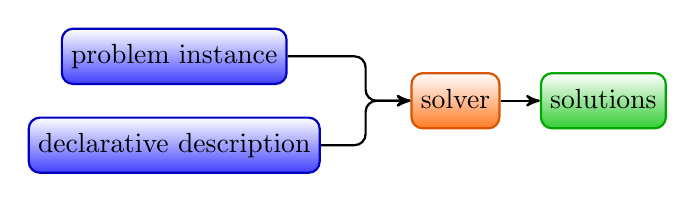
\begin{tikzpicture} [
			every rectangle node/.style={draw,rounded corners,text height=1.5ex,text depth=.25ex,minimum size=7mm},
			every path/.style={->,>=stealth',thick,rounded corners},
			node distance=5mm,
%			anchor=base,
			transform shape,
%			scale=0.8,%rotate=10,
		]
		
		\node[coordinate] (1) {};
		
		\node[rectangle,draw=maincolor!85!black,top color=white,bottom color=maincolor!85] (solver) [right=30mm of 1] {solver};
		\node[rectangle,draw=blue!75!black,top color=white,bottom color=blue!75] (instance) [above=2mm of 1] {problem instance};
		\node[rectangle,draw=blue!75!black,top color=white,bottom color=blue!75] (description) [below=2mm of 1] {declarative description};
		\node[rectangle,draw=green!65!black,top color=white,bottom color=green!75!black!80] (solutions) [right=of solver] {solutions};
		
		\node[coordinate] (2) at ($(description.east)!0.5!(solver.west)$) {};
		\node[coordinate] (3) at (instance.east -| description.east) {};
		\node[coordinate] (4) at ($(3)!0.5!(solver.west)$) {};
% 		
% 		\fill [red] (2) circle (2pt);
% 		\fill [red] (3) circle (2pt);
% 		\fill [red] (4) circle (2pt);
		
		\draw (instance) -| (4) |- (solver);
		\draw (description) -| (2) |- (solver);
		\draw (solver) -- (solutions);
		
	\end{tikzpicture}
	\end{center}
	
	\onslide<+->
	
	\begin{example}[encoding 3-coloring to SAT]
	
		\begin{itemize}
			\item Having a graph: \hspace{1.25cm}
				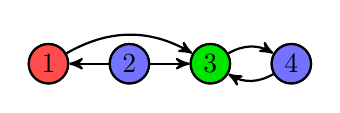
\begin{tikzpicture} [
						every circle node/.style={draw,inner sep=0,minimum size=5mm},
						every path/.style={->,>=stealth',thick},
						node distance=5mm,
			%			anchor=base,
						transform shape,
			%			scale=0.8,%rotate=10,
					]
					
					\node<2>[circle] (1) {1};
					\node<2>[circle] (2) [right=of 1] {2};
					\node<2>[circle] (3) [right=of 2] {3};
					\node<2>[circle] (4) [right=of 3] {4};
					\node<5->[circle,fill=red!70] (1) {1};
					\node<5->[circle,fill=blue!55] (2) [right=of 1] {2};
					\node<5->[circle,fill=green!90!black] (3) [right=of 2] {3};
					\node<5->[circle,fill=blue!55] (4) [right=of 3] {4};
					
					\draw (1) to [bend left] (3);
					\draw (2) to (1);
					\draw (2) to (3);
					\draw (3) to [bend left] (4);
					\draw (4) to [bend left] (3);
					
				\end{tikzpicture}
			
				
			\onslide<+->
			
			\item Instance:
				{\scriptsize$N = \set{1,2,3,4}$, $E = \set{\tuple{1,3}, \tuple{2,1}, \tuple{2,3}, \tuple{3,4}, \tuple{4,3}}$}
			
			\onslide<+->
			
			\item Encoding:
				
				{\scriptsize
				$\forall x \in N\ .\ green(x) \vee blue(x) \vee red(x)$\\
				$\forall x \in N\ .\ \neg(red(x) \wedge blue(x)) \wedge \neg(blue(x) \wedge green(x)) \wedge  \neg(green(x) \wedge red(x))$\\
				$\forall \tuple{x,y} \in E\ .\ \neg (red(x) \wedge red(y)) \wedge \neg (green(x) \wedge green(y)) \wedge \neg (blue(x) \wedge blue(y))$\\
				}
			
			\onslide<+->
			
			\item Solutions: {\scriptsize$I = \set{red(1), blue(2), green(3), blue(4)}$}, \ldots
			
		\end{itemize}
		
	\end{example}
	
	
\end{frame}

\begin{frame}{How Answer-Set Programming differs from SAT}
	\onslide<+->
	
	ASP is \structure{normal logic programs} under \structure{stable model semantics}.
	
	\onslide<+->
	
	\begin{definition}[normal logic program]
		A \structure{\emph{normal logic program}} is a set of rules $r$ of the form:
		\begin{center}
			$h \code{ :- } b_1 \code{,} \ldots \code{,}\ b_n \code{,}\ \code{not}\ b_{n+1} \code{,} \ldots \code{,}\ \code{not}\ b_m \code{.}$
		\end{center}
		where $\head{r} = \set{h}$ and $\body{r} = \set{b_1, \ldots, \code{not}\ b_m}$.
	\end{definition}
	
	In classical logic that would be
	\begin{center}
		$b_1 \wedge \ldots \wedge b_n \wedge \neg b_{n+1} \wedge \ldots \wedge \neg b_m \rightarrow h$
	\end{center}
	
\end{frame}

\begin{frame}{Stable Model Semantics}
	\onslide<+->
	
	\begin{definition}[active rules]
		\structure{\emph{Active rules}} of a program $P$ under an interpretation $I$ is the set
		\begin{center}
			$\activerules{I}{\prog} = \setcomp{r \in \prog}{I \models \body{r}}$
		\end{center}
	\end{definition}
	
	\begin{definition}[answer set]
		An interpretation $I$ is an \structure{\emph{answer set}} of a program $\prog$ iff\\
		$I$ is a minimal model of $\activerules{I}{\prog}$.
	\end{definition}
	
\end{frame}

\begin{frame}{Why minimal models 1/2}
	\onslide<+->
	
	\begin{itemize}
		\item Having the same graph: \hspace{0.25cm}
			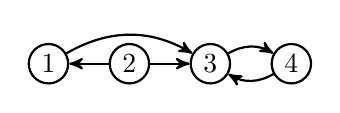
\begin{tikzpicture} [
					every circle node/.style={draw,inner sep=0,minimum size=5mm},
					every path/.style={->,>=stealth',thick},
					node distance=5mm,
		%			anchor=base,
					transform shape,
		%			scale=0.8,%rotate=10,
				]
				
				\node[circle] (1) {1};
				\node[circle] (2) [right=of 1] {2};
				\node[circle] (3) [right=of 2] {3};
				\node[circle] (4) [right=of 3] {4};
				
				\draw (1) to [bend left] (3);
				\draw (2) to (1);
				\draw (2) to (3);
				\draw (3) to [bend left] (4);
				\draw (4) to [bend left] (3);
				
			\end{tikzpicture} \hspace{\fill}
		
		\item Encoded by facts: \hfill \code{n(1). n(2). n(3). n(4).}\\
			\hfill \code{e(1,3). e(2,1). e(2,3). e(3,4). e(4,3).}
		
		\onslide<+->
		
		\item Program $\prog_{r,4}$ that finds all nodes reachable from $4$:
		
			\code{start(4).}\\
			\code{r(Y) :- start(X), e(X,Y).}\\
			\code{r(Y) :- r(X), e(X,Y).}
		
		\onslide<+->
		
		\item We want to get only models $I$, s.t.
			\begin{center}
				$\set{r(3), r(4)}\subseteq I\quad$ but $\quad\set{r(1), r(2)}\cap I = \emptyset$
			\end{center}
		
	\end{itemize}
	
\end{frame}

\begin{frame}{Why minimal models 2/2}
	\onslide<+->
	
	\begin{itemize}
		\item $\prog_{r,4}$ translated to classical logic
			\begin{center}
				$\begin{array}{rcl}
				start(X) \wedge e(X,Y) & \rightarrow & r(Y) \\
				r(X) \wedge e(X,Y) & \rightarrow & r(Y)
				\end{array}$
			\end{center}
		
		\item has also models containing $r(1)$ or $r(2)$.
		
		\onslide<+->
		
		\item We can add formulas
			\begin{center}
				$(\,start(X) \wedge e(X,Y)\,)\ \vee\ (\,r(X) \wedge e(X,Y)\,) \ \leftarrow \ r(Y)$
			\end{center}
		
		\onslide<+->
		
		\item but we still get
			\begin{center}
				$\begin{array}{rcl}
				r(2) \wedge e(2,1) & \rightarrow & r(1) \\
				(\,start(2) \wedge e(2,1)\,)\ \vee\ (\,r(2) \wedge e(2,1)\,) & \leftarrow & r(1)
				\end{array}$
			\end{center}
			that admits models with $r(1)$ and $r(2)$.
		
		\onslide<+->
		
		\item We want \structure{minimal models}.
		
	\end{itemize}
	
\end{frame}

\begin{frame}{Why only active rules}
	\onslide<+->
	
	\begin{itemize}
		\item The program $\prog_1$:
		\begin{center}
			$\code{p :- not}\ \code{q.}$\\
			$\code{q :- not}\ \code{p.}$
		\end{center}
		has minimal models \set{p}, \set{q}.
		
		\item But also the program $\prog_2$:
		\begin{center}
			$\code{p :- not}\ \code{q.}$
		\end{center}
		has minimal models \set{p}, {\color{red}\set{q}}.
		
		\onslide<+->
		
		\item Uder stable model semantics we get the following:
		\begin{itemize}
			\item $I_1 = \set{p}$, $\activerules{I_1}{\prog_1} = \set{\code{p:-not}\ \code{q.}}$, $I_1\models\activerules{I_1}{\prog_1}$ and $I_1$ is minimal\\
			\onslide<+->
			\item $I_2 = \set{p,q}$, $\activerules{I_2}{\prog_1} = \emptyset$, $I_2\models\activerules{I_2}{\prog_1}$ but so does $I_1 \subset I_2$\\
			\onslide<+->
			\item $I_3 = \set{q}$, $\activerules{I_3}{\prog_2} = \emptyset$, $I_3\models\activerules{I_3}{\prog_2}$ but so does $\emptyset \subset I_3$
		\end{itemize}
		
	\end{itemize}
	
\end{frame}

\begin{frame}{Obtaining an Answer Set}
	\onslide<+->
	
	\begin{center}
	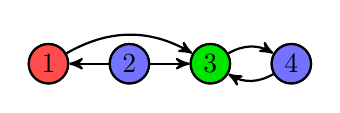
\begin{tikzpicture} [
			every circle node/.style={draw,inner sep=0,minimum size=5mm},
			every path/.style={->,>=stealth',thick},
			node distance=5mm,
%			anchor=base,
			transform shape,
%			scale=0.8,%rotate=10,
		]
		
		\node<1>[circle] (1) {1};
		\node<1>[circle] (2) [right=of 1] {2};
		\node<1>[circle] (3) [right=of 2] {3};
		\node<1>[circle] (4) [right=of 3] {4};
		\node<2->[circle,fill=red!70] (1) {1};
		\node<2->[circle,fill=blue!55] (2) [right=of 1] {2};
		\node<2->[circle,fill=green!90!black] (3) [right=of 2] {3};
		\node<2->[circle,fill=blue!55] (4) [right=of 3] {4};
		
		\draw (1) to [bend left] (3);
		\draw (2) to (1);
		\draw (2) to (3);
		\draw (3) to [bend left] (4);
		\draw (4) to [bend left] (3);
		
	\end{tikzpicture}
	\end{center}
	
	$\code{c(X,red)}\ \code{:-}\ \code{n(X), not}\ \code{c(X,green), not}\ \code{c(X,blue).}$\\
	$\code{c(X,green)}\ \code{:-}\ \code{n(X), not}\ \code{c(X,red), not}\ \code{c(X,blue).}$\\
	$\code{c(X,blue)}\ \code{:-}\ \code{n(X), not}\ \code{c(X,red), not}\ \code{c(X,green).}$\\
	$\code{:- e(X,Y),}\ \code{c(X,C),}\ \code{c(Y,C).}$
	
	\onslide<+->
	
	\begin{itemize}
		\item Guess: $I = \set{c(1,red), c(2,blue), c(3,green), c(4,red), \ldots}$
		
		\onslide<+->
		
		\item Check: $\activerules{I}{\prog} = \{$\\
			{\footnotesize
				\newcommand{\hs}{\hspace{0.05\textwidth}}%
				\hs$\code{c(1,red)}\ \code{:-}\ \code{n(1), not}\ \code{c(1,green), not}\ \code{c(1,blue).}$\\
				\hs$\code{c(4,red)}\ \code{:-}\ \code{n(4), not}\ \code{c(4,green), not}\ \code{c(4,blue).}$\\
				\hs$\code{c(3,green)}\ \code{:-}\ \code{n(3), not}\ \code{c(3,red), not}\ \code{c(3,blue).}$\\
				\hs$\code{c(2,blue)}\ \code{:-}\ \code{n(2), not}\ \code{c(2,red), not}\ \code{c(2,green).}$\\
			}
			$\}$
		
		\item $I\models\activerules{I}{\prog}$ and $I$ is minimal.
		
	\end{itemize}
	
\end{frame}



\section{Stepping}


\subsection{Stepping}

\begin{frame}{Introduction}% TODO: Adapt this frame
	\onslide<+->
	
	\begin{columns}[c]
	\column{0.7\textwidth}
		
		\begin{itemize}
			\item \structure{Answer-Set Programming} (ASP) is a declarative problem-solving paradigm
			\item Lack of development tools for ASP
			\onslide<+->
			\item \structure{MMDASP} @ TUW \alert{``The M\&M's of ASP''}
% 			\begin{itemize}
% 				\item by people in TUW, kbs
% 				\item development, testing, debugging, \ldots
% %	 			\item \url{www.kr.tuwien.ac.at/research/projects/mmdasp/}
% 			\end{itemize}
		\end{itemize}
		
	\column{0.3\textwidth}
		
		\includegraphics<2->[width=3cm]{nice_mm}
		
	\end{columns}
	
	
% 	\pause
	\onslide<+->
	
	
	\begin{columns}[b]
	\column{0.25\textwidth}

		\includegraphics<3->[width=5.2cm]{leo2-450-360}

	\column{0.75\textwidth}

		\begin{columns}[c]
		\column{0.62\textwidth}

			\begin{itemize}
				\item IDE for ASP \structure{SeaLion}
				\begin{itemize}
					\item plug-in for Eclipse
					\item \url{www.sealion.at}
				\end{itemize}
			\end{itemize}

		\column{0.38\textwidth}

			\includegraphics<3->[width=1.4cm]{eclipse}

		\end{columns}


% 		\pause
		\onslide<+->


		\begin{columns}[b]
		\column{0.15\textwidth}

		\column{0.8\textwidth}

			\begin{itemize}
				\item Declarative debugging happens to be impractical
% 				\begin{itemize}
% 					\item justifications
% 					\item Ouroboros
% 				\end{itemize}
				\onslide<+->
				\item \structure{Stepping} is a gradual evaluation of a program guided by the user
				\item Lifted to real-world languages and implemented for \sealion
			\end{itemize}

		\end{columns}

	\end{columns}
	
\end{frame}

\begin{frame}{Stepping in a Nutshell}
	\onslide<+->
	
	Having in mind: ``Answer-set is a minimal model of active rules.''
	
	\onslide<+->
	\begin{itemize}
		\item Stepping monotonically builds an Answer-Set
		\onslide<+->
		\begin{itemize}
			\item by filling a partial interpretation $I$ that is initially empty.
		\end{itemize}
		\onslide<+->
		\item Each step, a new active ground rule $r$ contributes to $I$
		\onslide<+->
		\begin{itemize}
			\item in order to satisfy its head $H(r)$.
		\end{itemize}
		\onslide<+->
		\item This activates more rules and the cycle continues.
		\onslide<+->
		\item If we maintain the property that $I$ is always an answer-set of
		the set $P$ of ground rules that already contributed,
		\onslide<+->
		\begin{itemize}
			\item when $P$ becomes all active rules, $I$ becomes an answer-set.
		\end{itemize}
	\end{itemize}
	
	\onslide+<+->{\vspace{10pt}

		Which rule contributes at a step?

		\onslide<+->
		User chooses -- Stepping is interactive
	}
	
\end{frame}

\newcommand{\hlt}[5]{%
	\alt<#2>{\colorbox{#1}{{\color{#1}$|$}#5}}{%
		\alt<#4>{\colorbox{#3}{{\color{#3}$|$}#5}}{%
			\colorbox{white}{{\color{white}$|$}#5}%
		}%
	}%
}%
\begin{frame}{A Simple Example}
	\onslide<1->
	
	\begin{columns}[t]
	\column{0.35\textwidth}
		
		\hlt{blue!30}{1}{green!60}{2-}{\texttt{a.}} \\
		\hlt{blue!30}{2,5}{green!60}{3}{\texttt{b :- a, not c.}} \\
		\hlt{blue!30}{2-4}{green!60}{5-}{\texttt{b :- a, not d.}} \\
		\hlt{blue!30}{1-3,5}{green!60}{4,6-}{\texttt{c.}}
		
	\column{0.15\textwidth}
		
		\begin{tabular}{r@{}l}
			$I=\{$ & \temporal<2>{$\}$}{$\texttt{a}\}$}{$\texttt{a},$} \\
			 & \onslide*<3,5>{$\texttt{b}\}$}\onslide*<4,6->{$\texttt{b},$} \\
			 & \onslide*<4,6>{$\texttt{c}\}$} \\
		\end{tabular}
		
	\column{0.5\textwidth}
		
		\begin{tabular}{r@{}l}
			$\prog=\{$ & \temporal<2>{$\}$}{$\texttt{a.}\}$}{$\texttt{a.},$} \\
			 & \onslide*<3>{$\texttt{b :- a, not c.}\}$}%
			   \onslide*<4>{$\alert{\texttt{b :- a, not c.}},$}%
			   \onslide*<5>{$\texttt{b :- a, not d.}\}$}%
			   \onslide*<6->{$\texttt{b :- a, not d.},$} \\
			 & \onslide*<4,6>{$\texttt{c.}\}$} \\
		\end{tabular}
		
	\end{columns}
	
	\vspace{20pt}
	key: \colorbox{blue!30}{{\color{blue!30}$|$}active rules{\color{blue!30}$|$}} \colorbox{green!60}{{\color{green!60}$|$}active rules occurring in $P${\color{green!60}$|$}}
	
\end{frame}

\begin{frame}{Real-World ASP Languages}
	\onslide<+->
	
	Theoretical stepping is defined for ground programs.
	
	\onslide<+->
	
	However, real-worlds ASP languages contain:
	
	\begin{itemize}
		\item arithmetics: $\code{maxrow(X):-}\ \code{row(X),}\ \code{not}\ \code{row(X+1).}$
		\onslide<+->
		\item comparison predicates: $\code{right\_top(X,Y):-}\ \code{row(X),}\ \code{col(Y),}\ \code{X<Y.}$
		\onslide<+->
		\item intervals: \code{row(1..4).}
		\onslide<+->
		\item aggregates: $\code{small:-}\ \code{\#count\{r(X):n(X)\}}\ \code{<}\ \code{5.}$
		\onslide<+->
		\item choice rules: $\code{1}\ \code{\{c(X,red),c(X,green),c(X,blue)\}}\ \code{1}\ \code{:-}\ \code{n(X).}$
	\end{itemize}
	
	\onslide<+->
	
	In my thesis I developed a theoretical framework that lifts Stepping to real-world ASP langugages
	and implemented it as a plugin for \sealion.
	
\end{frame}


\subsection{Demonstration}

\begin{frame}{Demonstration}
	
	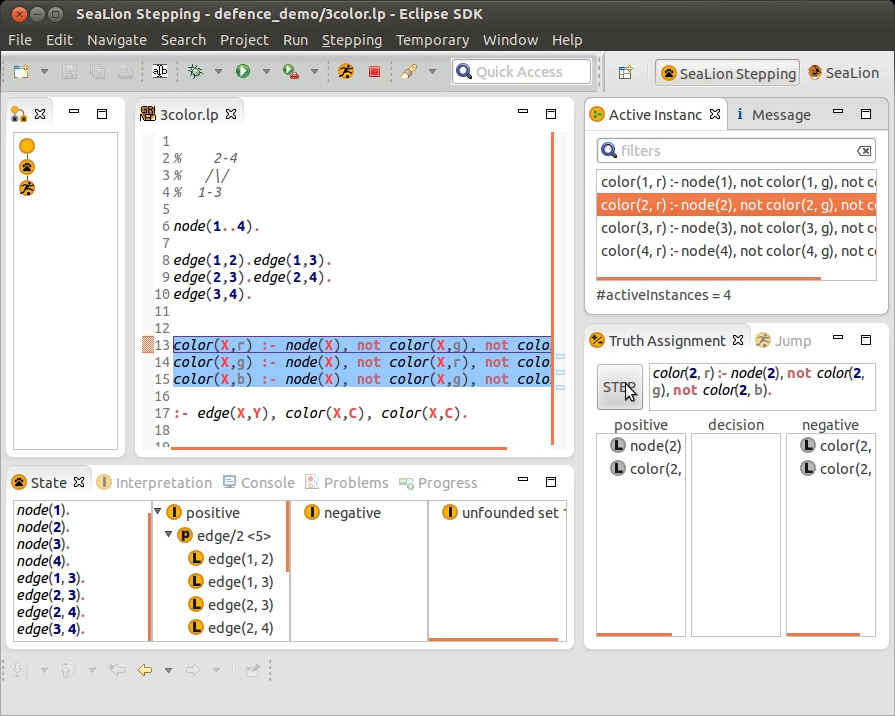
\includegraphics[width=\textwidth]{stepping_perspective}
	
\end{frame}



\section<presentation>*{Reference}


\subsection<presentation>*{Reference}

\begin{frame}{Reference}
	
% 	\bibliographystyle{plain}
% 	\bibliography{bibliography}{}
	
	\begin{thebibliography}{11}
	
	\small
	
	\beamertemplatearticlebibitems
	
	\bibitem{stepping}
		J. Oetsch, J. P{\"u}hrer, H. Tompits:
		\newblock Stepping Through an Answer-Set Program.
		\newblock {\em LPNMR}, 6645 (2011); 134--147.
	
	\bibitem{flp-for-acp}
		J. Oetsch, J. Pührer, H. Tompits:
		\newblock An FLP-Style Answer-Set Semantics for Abstract-Constraint Programs with Disjunctions
		\newblock {\em ICLP'12}, LIPIcs, 17 (2012); 222--234.
	
	\bibitem{DLstepping}
		J. Oetsch, J. Pührer, H. Tompits:
		\newblock Stepwise Debugging of Description-Logic Programs
		\newblock {\em LNCS}, 7265 (2012); 492--508.

	\bibitem{sealion13}
		P.-A. Busoniu, J. Oetsch, J. P{\"u}hrer, P. Skocovsky, H. Tompits:
		\newblock Sealion: An Eclipse-based IDE for Answer-Set Programming with Advanced Debugging Support
		\newblock {\em TPLP}, 13(4-5):657--673, 2013.
% 	
% 	\bibitem{FPL}
% 		W. Faber, G. Pfeifer, N. Leone:
% 		\newblock Semantics and complexity of recursive aggregates in answer set programming
% 		\newblock Artificial Intelligence 175 (1) (2011) 278–298.
	
	\end{thebibliography}
	
\end{frame}



\appendix



\section[Abstract-Constraint Semantics]{An FLP-Style Semantics for Abstract-Constraint Programs with Disjunctions}


\subsection[Abstract-Constraint Semantics]{An FLP-Style Semantics for Abstract-Constraint Programs with Disjunctions}

\begin{frame}{Abstract-Constraint Program \cite{flp-for-acp}}

	\begin{itemize}
		\item Only propositional level.
		\pause
		\item We use usual \structure{literals}.
		\pause
		\item \emph{Abstract-constraint atom} (\emph{\structure{c-atom}}) is a pair $A = \catom{D}{C}$.
		\begin{itemize}
			\item \emph{domain} $D$ is a set of literals (denoted $D_A$)
			\item \emph{satisfiers} $C \subseteq 2^D$ (denoted $C_A$)
		\end{itemize}
		\pause
		\item \emph{elementary} c-atom $\catom{\set{p}}{\set{\set{p}}}$ for standard literal $p$
		\pause
		\item \emph{\structure{Rule}} $r : A_1 | \ldots | A_k \colonminus A_{k+1}, \ldots, A_m, \text{not } A_{m+1}, \ldots, \text{not } A_n$.
		\begin{itemize}
			\item usual definitions of $H(r)$, $B(r)$, $B^+(r)$, $B^-(r)$, \emph{fact}, \emph{constraint}
			\item domain of a rule $r$ is $D_r = \bigcup_{A \in H(r) \cup B(r)} D_A$
		\end{itemize}
		\pause
		\item An \emph{\structure{interpretation}} $I$ is a consistent set of literals.
		\begin{itemize}
			\item $I$ \emph{satisfies} a c-atom $I \models \catom{D}{C}$ iff $I \cap D \in C$
			\item usual satisfaction of sets, rules and programs
		\end{itemize}
	\end{itemize}

	\pause

	\begin{example}[c-atom for an aggregate]
	\texttt{Gringo} aggregate \texttt{1\{a,b\}2}\newline
	turns into c-atom $\catom{\set{a,b}}{\set{\set{a}, \set{b}, \set{a,b}}}$.
	\end{example}

\end{frame}

\begin{frame}{Answer-Sets}

	\begin{itemize}
		\item A rule $r$ is \emph{\structure{active}} under $I$ iff $I \models B(r)$.
		\item Let $\Pi$ be a program, then \structure{$\Pi^I$} $= \setcomp{r \in \Pi}{I \models B(r)}$
		\item FLP (Faber, Pfeifer, Leone \cite{FPL}) answer-set is $I \models \Pi^I$ s.t.\newline
		there is no $I' \subset I$ that $I' \models \Pi^I$
		\pause
		\begin{itemize}
			\item There is, however, the mentioned minimisation problem. %TODO what kind of sentence is this ???
		\end{itemize}
	\end{itemize}

	\pause

	\begin{definition}[answer-set]
	Let $\Pi$ be an abstract-constraint program and $I$ an interpretation.\newline
	\pause
	$I$ is an \emph{\structure{answer-set}} of $\Pi$ if $I \models \Pi^I$ and there is no $I' \subset I$ such that\newline
	\pause
	for every $r \in \Pi^I$ with $I' \models B(r)$ there is some $A \in H(r)$ with
	$I' \models A$ and $I' \cap D_A = I \cap D_A$.
	\end{definition}

\end{frame}

\begin{frame}{Example (1/2)}

	\ldots\ there is no $I' \subset I$ such that for every $r \in \Pi^I$ with $I' \models B(r)$ there is some $A \in H(r)$ with
	$I' \models A$ and $I' \cap D_A = I \cap D_A$.

	\begin{example}[1]
	Consider program $\Pi_1$ containing single fact
	$$\catom{\set{a,b}}{\set{\set{a}, \set{b}, \set{a,b}}}.$$
	We want the answer-sets to be
	$$\set{a}, \set{b} \text{ and } \set{a,b}.$$
	FLP semantics rules out $\set{a,b}$, because $\set{a} \subset \set{a,b}$, but\newline
	our semantics does not, because $\set{a} \cap D_A \neq \set{a,b} \cap D_A$.
	\end{example}

\end{frame}

\begin{frame}{Example (2/2)}

	\ldots\ there is no $I' \subset I$ such that for every $r \in \Pi^I$ with $I' \models B(r)$ there is some $A \in H(r)$ with
	$I' \models A$ and $I' \cap D_A = I \cap D_A$.

	\begin{example}[2]
	Consider program $\Pi_2$ containing single fact
	$$\catom{\set{a,b}}{\set{\set{a}, \set{b}, \set{a,b}}} \ |\  \catom{\set{a,c}}{\set{\set{a,c}}}.$$
	The answer-sets are again $\set{a}$, $\set{b}$ and $\set{a,b}$, but \textbf{not} $\set{a,c}$,\newline
	because $I' = \set{a}$ satisfies $A = \catom{\set{a,b}}{\set{\set{a}, \set{b}, \set{a,b}}}$\newline
	and $I' \cap D_A = \set{a,c} \cap D_A$.
	\end{example}

	\pause

	\begin{itemize}
		\item minimisation only between c-atoms with different domains.
	\end{itemize}

\end{frame}

\begin{frame}{Unfounded Sets}

	\begin{definition}[external support]
	Let $r$ be a rule, $X$ a set of literals, and $I$ an interpretation\\
	such that $X \subseteq I$ and $I \models r$.\\
	Then, $r$ is an \emph{\structure{external support}} for $X$ with respect to $I$ iff
	\begin{itemize}
		\item $I \models B(r)$,
		\item $I \setminus X \models B(r)$,
% 		\item $\exists A \in H(r) \ .\  \exists S \in C_A$ with $X \cap D_A \neq \emptyset$ and
% 		$I \cap D_A \subseteq S$,
% 		\item $\forall A \in H(r)$ with $I \models A$ we have $X \cap I \cap D_A \neq \emptyset$.
		\item $\forall A \in H(r)$ with $I \models A$ we have $X \cap D_A \neq \emptyset$.
	\end{itemize}
	\end{definition}

	\pause

	\begin{itemize}
		\item $X$ is \emph{\structure{unfounded}} in $\Pi$ w.r.t. $I$ iff it has no external support.
		\item $I$ is an answer-set of $\Pi$ iff $I \models \Pi$ and there are no unfounded sets in $I$ (except $\emptyset$).
	\end{itemize}

\end{frame}



\section[Advanced Stepping]{Stepping Through an Abstract-Constraint Programs}


\subsection[Advanced Stepping]{Stepping Through an Abstract-Constraint Programs}

\begin{frame}{Stepping Through an Abstract-Constraint Programs}

	\begin{itemize}
		\item Building an answer-set monotonically
		\item Activating ground rules
		\item Ensure that what we end up with is an answer-set
	\end{itemize}

\end{frame}

\begin{frame}{State}

	\begin{definition}[state structure]
	A \emph{\structure{state structure}} $S$ is a tuple $\langle P, I, I^-, \Upsilon \rangle$, where
	\begin{itemize}
		\item $P$ is a set of ground rules (denoted $P_S$),
		\item $I$ is an interpretation (denoted $I_S$),
		\item $I^-$ is a set of literals disjoint with $I$ (denoted $I^-_S$),
		\item $\Upsilon$ is a set of sets of literals (denoted $\Upsilon_S$).
	\end{itemize}
	$D_S = I \cup I^-$ is the domain of $S$.
	\end{definition}

	\pause

	\begin{definition}[state]
	A state structure $S = \langle P, I, I^-, \Upsilon \rangle$ is a \emph{\structure{state}} iff
	\begin{itemize}
		\item $I \models B(r)$ and $I \models r$ for every $r \in P$,
		\item $D_r \subseteq D_S$ for every $r \in P$,
		\item $\Upsilon = \setcomp{X \subseteq I}{X\text{ is unfounded in }P\text{ w.r.t. }I}$.
	\end{itemize}
	\end{definition}

\end{frame}

\begin{frame}{More on States}

	\begin{itemize}
		\item An \emph{\structure{empty state}} $S = \langle \emptyset, \emptyset, \emptyset, \set\emptyset \rangle$ is a state.
		\item A state $S$ is \emph{\structure{stable}} iff $I_S$ is an answer-set of $P_S$.
		\item $S$ is stable iff $\Upsilon_S = \set\emptyset$.
	\end{itemize}

	\pause

	\begin{example}
	Remember the \texttt{DLV} program \texttt{ a|b. a:-b. b:-a.}\\
	\pause
	After stepping through the fact, we get to the state
	$$\langle \set{\texttt{a|b.}}, \set{a,b}, \emptyset, \set{\emptyset,\set{a},\set{b}} \rangle$$
	that is unstable.
	\pause
	But stepping through the other rules supports the unfounded sets.
	$$\langle \set{\texttt{a|b.a:-b.}}, \set{a,b}, \emptyset, \set{\emptyset,\set{b}} \rangle$$
	$$\langle \set{\texttt{a|b.a:-b.b:-a.}}, \set{a,b}, \emptyset, \set{\emptyset} \rangle$$
	\end{example}

\end{frame}

\begin{frame}{Successor}

	\begin{definition}[successor]
	$S' = \langle P', I', I'^-, \Upsilon' \rangle$ is a \emph{\structure{successor}} of $S = \langle P, I, I^-, \Upsilon \rangle$ iff\newline
	there is a rule $r \in P' \setminus P$ and sets $\Delta, \Delta^- \subseteq D_r$ s.t.
	\begin{itemize}
		\item $P' = P \cup \set{r}$,
		\item $I' = I \cup \Delta$, $I'^- = I^- \cup \Delta^-$ and $D_S \cap (\Delta \cup \Delta^-) = \emptyset$,
		\item $D_r \subseteq D_{S'}$,
		\item $I \models B(r)$,
		\item $I' \models B(r)$ and $I' \models r$,
		\item $X' \in \Upsilon'$ iff $X' = X \cup \Delta'$, where
		$X \in \Upsilon$, $\Delta' \subseteq \Delta$ and
		$r$ is not an external support for $X'$ w.r.t. $I'$.
	\end{itemize}
	\end{definition}

	\pause

	\begin{example}[s]
	See the demonstration\ldots
	\end{example}

\end{frame}

\begin{frame}{Computation}

	\begin{itemize}
		\item A \emph{\structure{computation}} is a sequence of successors.
		\pause
		\begin{theorem}[Soundness]
			Let $\Pi$ be a program and $S$ a state such that\newline
			$P_S = \Pi^{I_S}$ and $\Upsilon_S = \set\emptyset$, then
			$I_S$ is an answer-set of $\Pi$.
		\end{theorem}
		\pause
		\begin{theorem}[Completeness]
			Let $\Pi$ be a program and $S_0$ a state with $P_{S_0} \subseteq \Pi$ and\newline
			$I$ an answer-set of $\Pi$ with $I_{S_0} \subseteq I$ and $I^-_{S_0} \cap I = \emptyset$, then\newline
			there is a computation starting in $S_0$ and ending in stable $S_n$ with
			$P_{S_n} = \Pi^I$ and $I_{S_n} = I$.
		\end{theorem}
		\pause
		\item The empty state is a stable state of any program.
		\item Every stable state is reachable from the empty state.
	\end{itemize}

\end{frame}



\section{Demonstration}


\subsection{Demonstration}

\begin{frame}{Demonstration}

	\begin{center}
		Demonstration \ldots
	\end{center}

\end{frame}



\section{Breakpoints}


\subsection{Breakpoints}

\begin{frame}{Jump}

	\begin{block}{Proposition}
		Let $\Pi$ be a program, $\Pi' \subseteq \Pi \cup \funid{gr}(\Pi)$ and
		$I$ an answer-set of $\Pi'$.\\
		Then $\langle \funid{gr}(\Pi')^I, I, \bigcup_{r \in \funid{gr}(\Pi')^I} D_r \setminus I, \set\emptyset \rangle$ is a state.
	\end{block}

	\pause

	\begin{itemize}
		\item Being in state $\langle P, I, I^-, \Upsilon \rangle$,
		\item compute answer-set $I'$ of
		\begin{itemize}
			\item $\Pi' = ($rules selected for jumping $\cup\ P)\ \cup$
			\item $\setcomp{\texttt{:-not}\ a\texttt{.}}{a \in I} \cup \setcomp{\texttt{:-}\ a\texttt{.}}{a \in I^-}$.
% 			\item $\setcomp{\colonminus not\ a.}{a \in I} \cup \setcomp{\colonminus a.}{a \in I^-}$,
		\end{itemize}
		\item Then the new state is $\langle P', I', I'^-, \set\emptyset \rangle$, where
		\begin{itemize}
			\item $P' = \funid{gr}(\Pi')^{I'}$ and
			\item $I'^- = \bigcup_{r \in P'} D_r \setminus I$
		\end{itemize}
	\end{itemize}

\end{frame}



\section<presentation>*{Reference}


\subsection<presentation>*{Reference}

\begin{frame}{Reference}

	\begin{thebibliography}{11}

	\small

	\beamertemplatearticlebibitems
%
% 	\bibitem{stepping}
% 		J. Oetsch, J. P{\"u}hrer, H. Tompits:
% 		\newblock Stepping Through an Answer-Set Program.
% 		\newblock {\em LPNMR}, 6645 (2011); 134--147.
%
% 	\bibitem{flp-for-acp}
% 		J. Oetsch, J. Pührer, H. Tompits:
% 		\newblock An FLP-Style Answer-Set Semantics for Abstract-Constraint Programs with Disjunctions
% 		\newblock {\em ICLP'12}, LIPIcs, 17 (2012); 222--234.
%
% 	\bibitem{DLstepping}
% 		J. Oetsch, J. Pührer, H. Tompits:
% 		\newblock Stepwise Debugging of Description-Logic Programs
% 		\newblock {\em LNCS}, 7265 (2012); 492--508.
%
% 	\bibitem{sealion13}
% 		P.-A. Busoniu, J. Oetsch, J. P{\"u}hrer, P. Skocovsky, H. Tompits:
% 		\newblock Sealion: An Eclipse-based IDE for Answer-Set Programming with Advanced Debugging Support
% 		\newblock {\em TPLP}, 13(4-5):657--673, 2013.

	\bibitem{FPL}
		W. Faber, G. Pfeifer, N. Leone:
		\newblock Semantics and complexity of recursive aggregates in answer set programming
		\newblock Artificial Intelligence 175 (1) (2011) 278–298.

	\end{thebibliography}
%
% 	\begin{thebibliography}{10}
%
% 	\beamertemplatearticlebibitems
%
% 	\bibitem{semantics}
% 		J. Oetsch, J. Pührer, H. Tompits:
% 		\newblock An FLP-Style Answer-Set Semantics for Abstract-Constraint Programs with Disjunctions
% 		\newblock ICLP 2012, LIPIcs, 17 (2012); 222-234.
%
% 	\bibitem{dlstepping}
% 		J. Oetsch, J. Pührer, H. Tompits:
% 		\newblock Stepwise Debugging of Description-Logic Programs
% 		\newblock In: Correct Reasoning - Essays on Logic-Based AI in Honour of Vladimir Lifschitz,
% 		LNCS, 7265 (2012); 492-508.
%
% 	\bibitem{FPL}
% 		W. Faber, G. Pfeifer, N. Leone:
% 		\newblock Semantics and complexity of recursive aggregates in answer set programming
% 		\newblock Artificial Intelligence 175 (1) (2011) 278–298.
%
% 	\end{thebibliography}

\end{frame}

\begin{frame}{The End}

	\begin{center}
% 		\includegraphics[width=5cm]{leoParrotWide-450x360r}

		\vspace{5pt}

		Please, try out \structure{Stepping} in \structure{SeaLion}\\
		and tell us what you think.

		\vspace{5pt}

		\url{www.sealion.pt}\\

		\vspace{5pt}

		\texttt{aifargonos@gmail.com}
	\end{center}
%
% 	\begin{columns}[c]
% 	\column{0.5\textwidth}
%
% 		Please, try out \structure{Stepping} in \structure{SeaLion}\\
% 		and tell us what you think.
%
% 		\vspace{10pt}
%
% 		\url{www.sealion.pt}\\
% 		\texttt{aifargonos@gmail.com}
%
% 	\column{0.45\textwidth}
%
% 		\includegraphics[width=5cm]{leoParrotWide-450x360r}
%
% 	\end{columns}

\end{frame}



\end{document}